\documentclass[10pt,twocolumn,letterpaper]{article}
%% Welcome to Overleaf!
%% If this is your first time using LaTeX, it might be worth going through this brief presentation:
%% https://www.overleaf.com/latex/learn/free-online-introduction-to-latex-part-1

%% Researchers have been using LaTeX for decades to typeset their papers, producing beautiful, crisp documents in the process. By learning LaTeX, you are effectively following in their footsteps, and learning a highly valuable skill!

%% The \usepackage commands below can be thought of as analogous to importing libraries into Python, for instance. We've pre-formatted this for you, so you can skip right ahead to the title below.

%% Language and font encodings
\usepackage[spanish,english]{babel}
\usepackage[utf8x]{inputenc}
\usepackage[T1]{fontenc}

%% Sets page size and margins
\usepackage[a4paper,top=3cm,bottom=2cm,left=3cm,right=3cm,marginparwidth=1.75cm]{geometry}

%% Useful packages
\usepackage{amsmath}
\usepackage{graphicx}
\usepackage[colorinlistoftodos]{todonotes}
\usepackage[colorlinks=true, allcolors=blue]{hyperref}
\usepackage{algorithm}  
\usepackage{algpseudocode}  
\usepackage{amsmath}  
\renewcommand{\algorithmicrequire}{\textbf{Input:}}  % Use Input in the format of Algorithm  
\renewcommand{\algorithmicensure}{\textbf{Output:}} % Use Output in the format of Algorithm  
\usepackage{listings}
\usepackage{float}

 \lstset{ %
    language=Octave,                % the language of the code
    basicstyle=\footnotesize,           % the size of the fonts that are used for the code
    numbers=left,                   % where to put the line-numbers
    numberstyle=\tiny\color{gray},  % the style that is used for the line-numbers
    stepnumber=2,                   % the step between two line-numbers. If it's 1, each line 
                                    % will be numbered
    numbersep=5pt,                  % how far the line-numbers are from the code
    backgroundcolor=\color{white},      % choose the background color. You must add \usepackage{color}
    showspaces=false,               % show spaces adding particular underscores
    showstringspaces=false,         % underline spaces within strings
    showtabs=false,                 % show tabs within strings adding particular underscores
    frame=single,                   % adds a frame around the code
    rulecolor=\color{black},        % if not set, the frame-color may be changed on line-breaks within not-black text (e.g. commens (green here))
    tabsize=2,                      % sets default tabsize to 2 spaces
    captionpos=b,                   % sets the caption-position to bottom
    breaklines=true,                % sets automatic line breaking
    breakatwhitespace=false,        % sets if automatic breaks should only happen at whitespace
    title=\lstname,                 % show the filename of files included with \lstinputlisting;
                                    % also try caption instead of title
    keywordstyle=\color{blue},          % keyword style
    commentstyle=\color{dkgreen},       % comment style
    stringstyle=\color{mauve},         % string literal style
    escapeinside={\%*}{*)},            % if you want to add LaTeX within your code
    morekeywords={*,...}               % if you want to add more keywords to the set
}

%% Title
\title{
		%\vspace{-1in} 	
		\usefont{OT1}{bch}{b}{n}
		\normalfont \normalsize \textsc{CS303 Artifical Intelligence} \\ [10pt]
		\huge Gomoku Project \\
}

\usepackage{authblk}

\author[1]{Hu yubin, 11712121}

\affil[1]{\small{Department of Computer Science and Engineering, Southern University of Science and Technology}}

\begin{document}
\maketitle

\selectlanguage{english}
\begin{abstract}
This project is implementing a Gomuku AI that can play on a specified platform with other AI.
\end{abstract} \\ 
\\ 
{\textbf{Keywords} \\
Gomoku, AI, Search tree }

\section{Preliminaries}
Gomoku, also called Five in a Row, is an abstract strategy board game. It is traditionally played with Go pieces (black and white stones) on a chessboard. The chessboard is initially in size of $15 \times 15$\cite{Case1971Gomoku}. This project need us to implement the AI algorithm of Gomoku according to the interface requirements and submit it to the system as required for usability testing, points race, and round robin. The use of memory cannot go beyond 100M, the time to find a place to drop cannot be longer than 5s, the whole battle cannot take longer than 180s.

\subsection{Software}
The code of Gomoku is written in Python. Version is Python 3.7.4. And only \emph{numpy} package is extra imported.

For analytics section, I use \emph{math}, \emph{time} and \emph{random} packages as tools to test the strength of AI.

\subsection{Algorithm}
The main algorithm is minimax seach tree, depth-first-search, $\alpha$-$\beta$ pruning algorithms, heuristic strategy for calculate the scores and Aho-Corasick automata\cite{Aho1975Efficient} in some version.

\section{Methodology}
The basic implementation is minimax tree, all the optimization is based on it. For the correction, I design the evaluation function and some special judge to find the better way to go the pieces. For time and space limit, I do $\alpha$-$\beta$ pruning algorithms,  heuristic strategy, global and local search\cite{M2001Global} and some other optimizations. 

\subsection{Representation}

\begin{itemize}
    \item 
    \emph{Chess}
    \begin{itemize}
        \item 
        COLOR\_BLACK = -1\\
        This is a constant. "-1" represents blank chess
    \end{itemize}
    \begin{itemize}
        \item 
        COLOR\_White = 1\\
        This is a constant. "1" represents white chess
    \end{itemize}
    \begin{itemize}
        \item 
        COLOR\_NONE = 0\\
        This is a constant. "0" represents that there is no chess
    \end{itemize}
\end{itemize}
\begin{itemize}
    \item 
    \emph{shape}
    \begin{align*}
        = &\{'h5': 20000,~# Win\\ 
        &'h4': 2000,~\# Alive4\\
        &'t4': 450,~\# Jump4\\
        &'h3': 450,~\# Alive3\\
        &'c4': 300,~\# Rush4\\
        &'t3': 300,~\# Jump3\\
        &'h2': 100,~\# Alive2\\
        &'c3': 50,~\# Rush3\\
        &'c2': 20\}~\# Rush2\\
    \end{align*}
    This is a dictionary. It represents different chess pattern and their scores. The higher, the better.
\end{itemize}
\begin{itemize}
    \item 
    \emph{totleTime}
    This is a double parameter. It records the time that the AI used.
\end{itemize}
\begin{itemize}
    \item 
    \emph{candidate\_list}
    This is a list. It records the steps that AI will go. We choose the last step as AI's best step. 
\end{itemize}
\begin{itemize}
    \item 
    \emph{Depth}
    This is a integer parameter. It is the depth of the minimax search tree. It may be changed because of the time limit.
\end{itemize}
\begin{itemize}
    \item 
    \emph{sortedNum}
    This is a integer parameter. It is the number of the steps in each depth of the minimax search tree. I will evaluate every the single point from both players and sort them by the calculated score.
\end{itemize}
\begin{itemize}
    \item 
    \emph{empty}
    This is a list. It is the empty chessboard.
\end{itemize}
\begin{itemize}
    \item 
    \emph{myScore}
    This is a integer parameter. It records the current score of AI.
\end{itemize}
\begin{itemize}
    \item 
    \emph{enemyScore}
    This is a integer parameter. It records the current score of AI's enemyScore.
\end{itemize}
\begin{itemize}
    \item 
    \emph{totalScore}
    This is a integer parameter. It records the current score of both players.
\end{itemize}
\begin{itemize}
    \item 
    \emph{level}
    This is a 15 $\times$ 15 list. I think the pieces in the middle is better in the same case. So that it is added to the score with small impact.
\end{itemize}

\subsection{Architecture}
There are several different versions of AI, some of them use different implementations. So that I will show them separately.

\begin{itemize}
    \item
    \emph{AI}
    \begin{itemize}
        \item
        \emph{init} 
        Initialize some parameters, such as timeout, chessboard status, minimax search tree's depth, candidate-list, two players' status and scores and score table. Especially, I designed AI for black and AI for white, They has the same modes of thought. But for timeout, and search ability, I give them different parameters to achieve better performance.
    \end{itemize}
    \begin{itemize}
        \item 
        \emph{go}
        judge the first step for blank and white. If AI is blank, it will choose (7, 7) directly. If AI is white, it will choose on of (6, 6), (6, 8), (8, 8), (8, 6) randomly. Otherwith, \emph{go} will put all the candidates steps searched by \emph{minimax} to the candidate list for the given chessboard. Especially, for test case, I judeg whether the given chessboard is a test case or not by count the number of chess. If the different between the history and the given chessboard is over one, I guess it is a test case and do the optimization on it.
    \end{itemize}
    \begin{itemize}
        \item 
        \emph{minimax}
        The main function in this project, it is a minimax search tre to find the steps that AI will go. It divides into black part and white part.
    \end{itemize}
    \begin{itemize}
        \item 
        \emph{count\_chess\_number}
        Count the number of chesses in the current chessboard.
    \end{itemize}
    \begin{itemize}
        \item 
        \emph{evaluation\_point}
        Evaluate the single point's score in the current chessboard.
    \end{itemize}
    \begin{itemize}
        \item 
        \emph{evaluation\_global}
        Evaluate the global score in the current chessboard. It depends on all the single point's score.
    \end{itemize}
    \begin{itemize}
        \item 
        \emph{evaluation\_line}
        Evaluate the score of a specified length line.
    \end{itemize}
    \begin{itemize}
        \item 
        \emph{next\_step}
        Generate the top 5 steps for AI to run the minimax search tree.
    \end{itemize}
    \begin{itemize}
        \item 
        \emph{update\_score}
        Update \emph{myScore}, \emph{enemyScore} and \emph{totalScore} after a step is choosed in the minimax tree.
    \end{itemize}
\end{itemize}

In another version, I use Aho-Corasick automata to find the pattern in the chessboard.

\begin{itemize}
    \item 
    \emph{Node}
    \begin{itemize}
        \item 
        \emph{init}
        Initialize next, fail, isword and word.
    \end{itemize}
\end{itemize}
\begin{itemize}
    \item 
    \emph{automata}
    \begin{itemize}
        \item 
        \emph{add}
        Add the pattern into the automata.
    \end{itemize}
    \begin{itemize}
        \item 
        \emph{make\_fail}
        Build the automata by the patterns that I added before.
    \end{itemize}
    \begin{itemize}
        \item 
        \emph{search}
        Search which pattern appear the in a specified line.
    \end{itemize}
\end{itemize}

\subsection{Mode design}

\begin{figure}[H]
  \centering
  % Requires \usepackage{graphicx}
  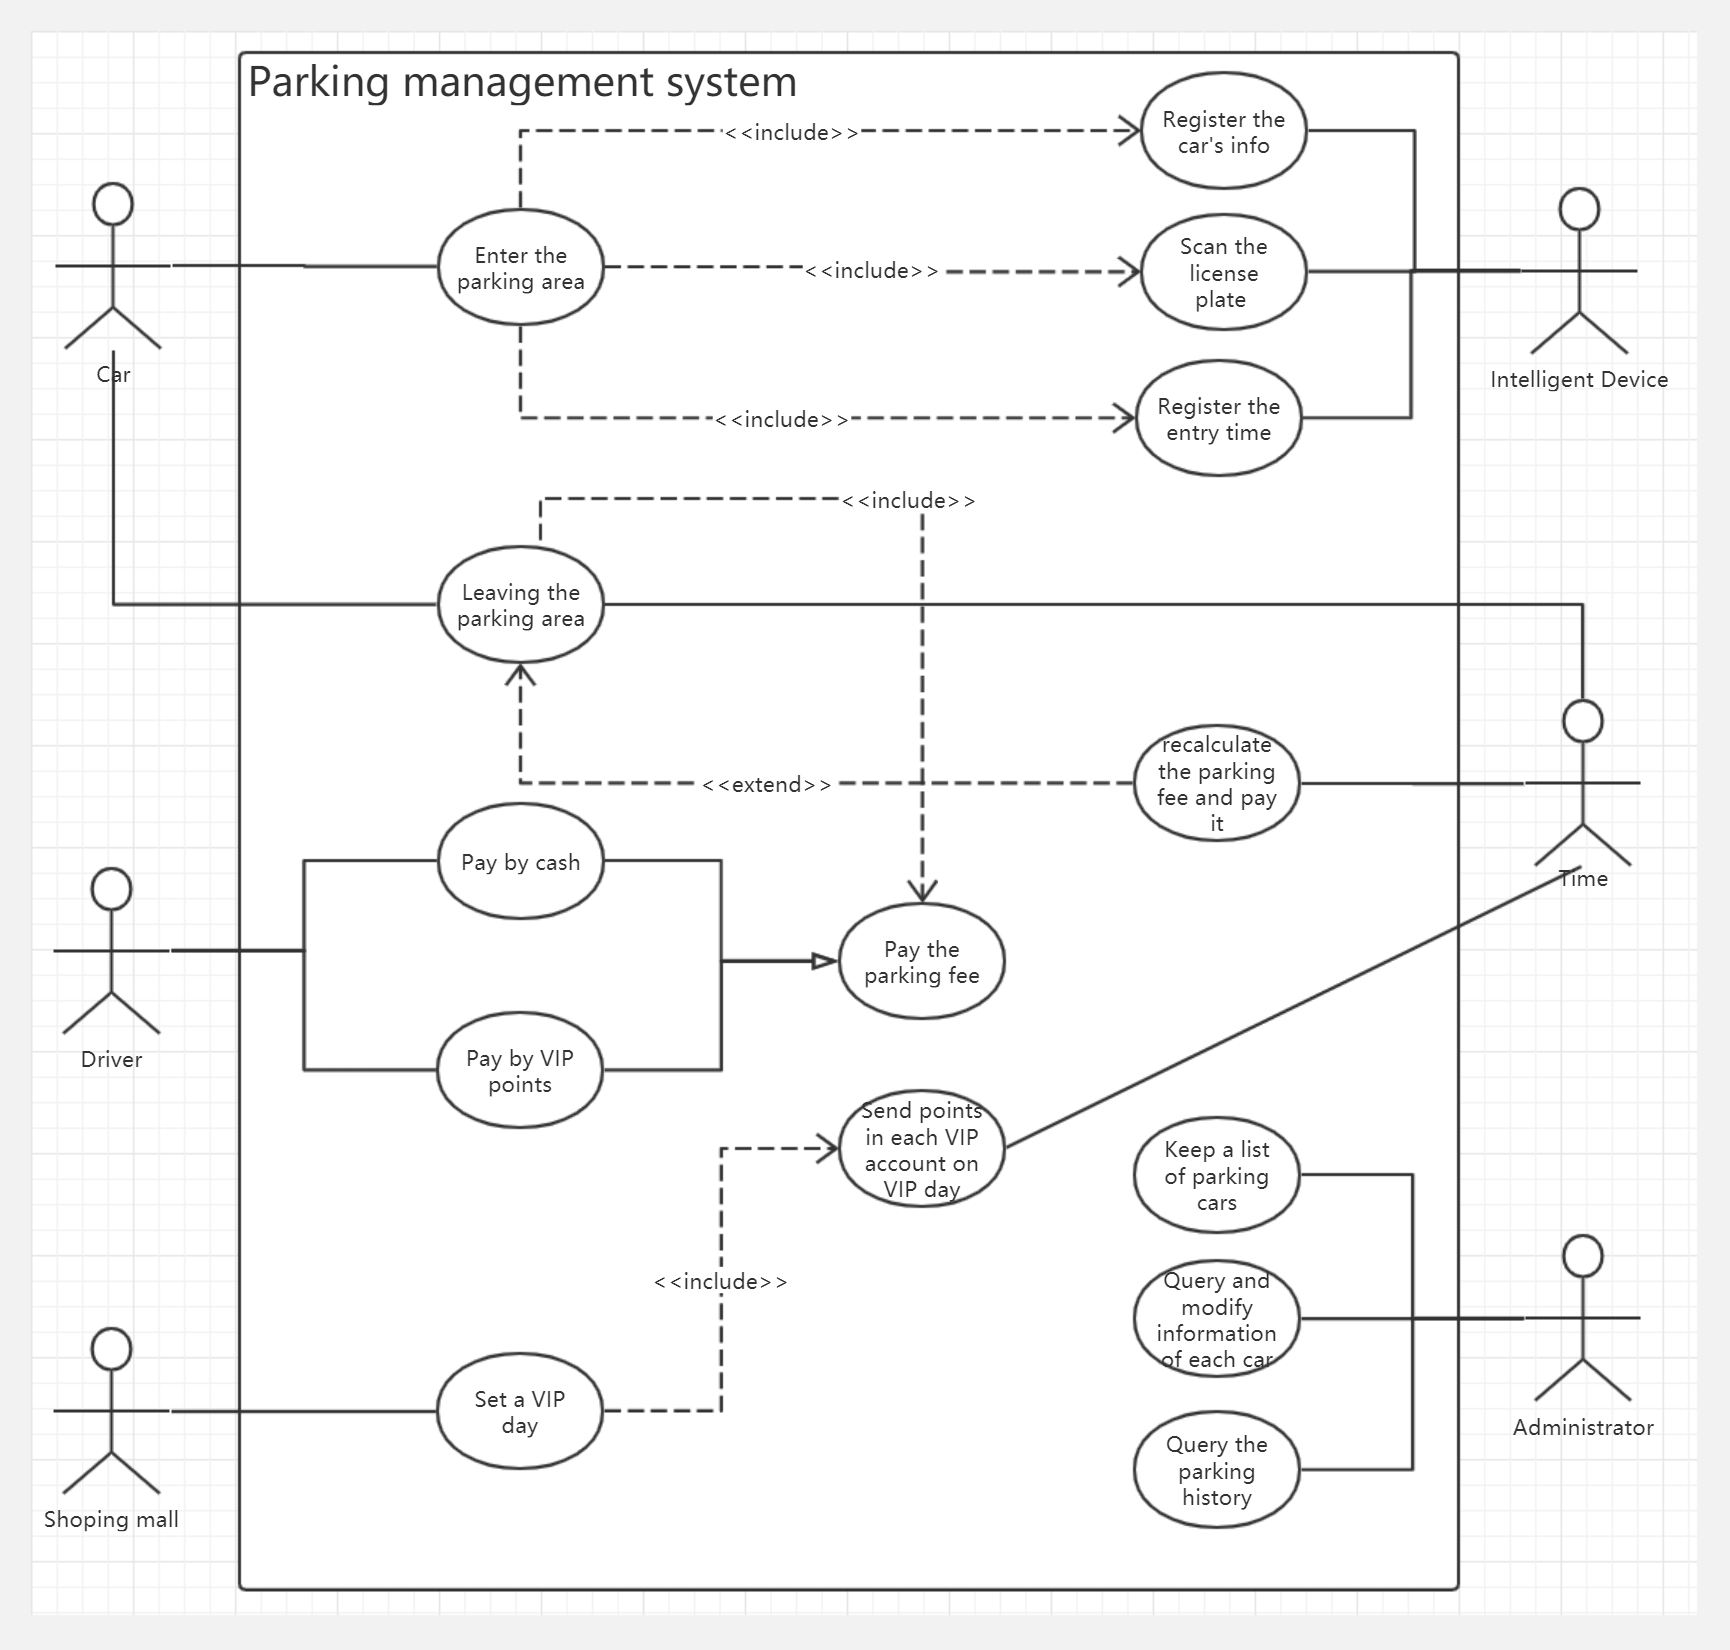
\includegraphics[width=0.4\textwidth]{Fig1.png}\\
  \caption{Mode design diagram
}\label{straddltimeScale}
\end{figure}

The flow chart of Gomoku project is shown in \emph{Figure 1}.

\subsection{Detail of Algorithm}

\subsubsection{minimax search tree}
When dealing with gains, it is referred to as "maximin"—to maximize the minimum gain. Originally formulated for two-player zero-sum game theory, covering both the cases where players take alternate moves and those where they make simultaneous moves, it has also been extended to more complex games and to general decision-making in the presence of uncertainty.\\

For Gomoku, we set the depth of minimax search tree and the number of node in each depth. Due to the time limitation, I set the depth to 5 and the number of node to 5 when AI is blank. And I set the depth to 4 and the number of node to 7 when AI is White.

\begin{algorithm}
  \caption{minimax seqarch tree}
  \begin{algorithmic}[1]
    \Function {MINIMAX}{node, depth, maxAI}
        \If {depth == 0 or point is a terminal point}
            \Return evaluation of point
        \EndIf
        \If {maxAI}
            \State maxEva = -inf
            \For {each candidate}
                \State eva = minimax(candidate, depth-1, false)
            \EndFor
            \State maxEva = max(maxEva, eva)
            \State \Return maxEva
        \Else
            \State minEva = inf
            \For {each candidate}
                \State eva = minimax(candidate, depth-1, true)
            \EndFor
            \State minEva = min(minEva, eva)
            \State \Return minEva
        \EndIf
    \EndFunction  
  \end{algorithmic}  
\end{algorithm}

\subsubsection{$\alpha$-$\beta$ pruning algorithms}
Alpha–beta pruning is a search algorithm that seeks to decrease the number of nodes that are evaluated by the minimax algorithm in its search tree. It stops evaluating a move when at least one possibility has been found that proves the move to be worse than a previously examined move. 

\begin{algorithm}
  \caption{$alpha$-$beta$ pruning}
  \begin{algorithmic}[1]
    \If{maxAI}
        \If score > alpha
            \State alpha = score
        \EndIf
        \If alpha >= beta:
            \State \Return alpha
        \EndIf
        \State \Return alpha
    \Else
        \If score < beta:
            \State beta = score
        \EndIf
        \If alpha >= beta:
            \State \Return beta
        \EndIf
        \State \Return beta
    \EndIf
  \end{algorithmic}  
\end{algorithm} 

\subsubsection{evaluation\_line}
I find that a chess only affect at most 32 chesses in the chessboard.

\begin{figure}[H]
  \centering
  % Requires \usepackage{graphicx}
  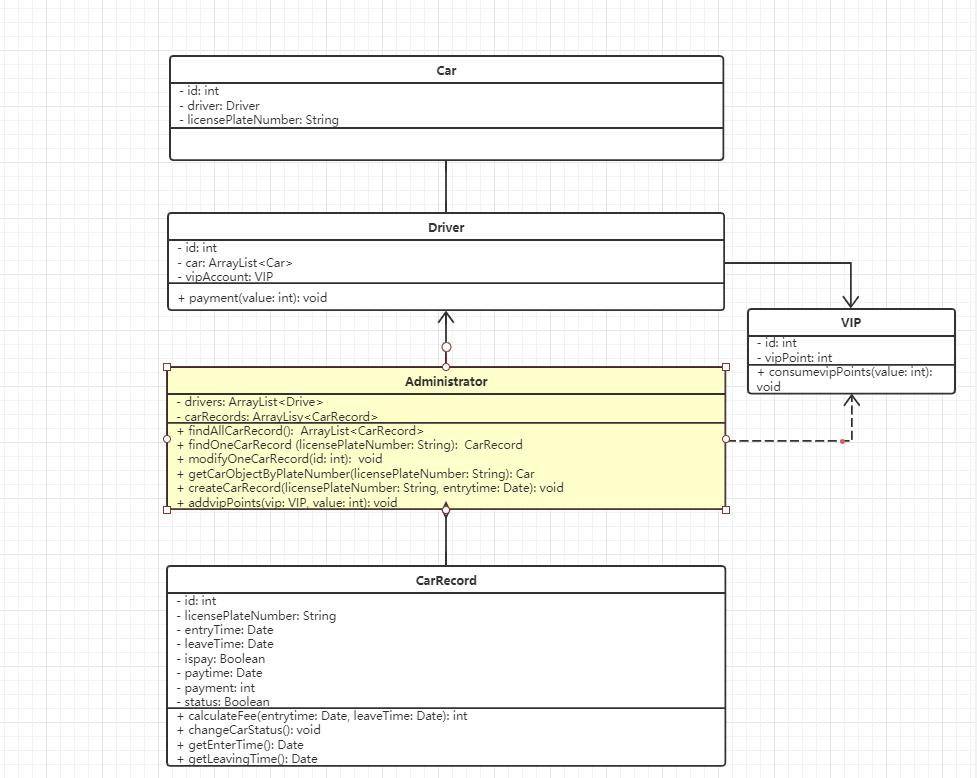
\includegraphics[width=0.4\textwidth]{Fig2.png}\\
  \caption{32 affected chesses
}\label{straddltimeScale}
\end{figure}

\subsubsection{Heuristic Search}
I evaluate the point in two ways. One is the score that the AI color chess is in the point, the other is the opponent color chess in the point. The sum of them is the final score of the point. I consider both of them because the point that benefits opponent also should be taken into account.

Due to the time limitation, I only choose 5 candidates in each depth.

\begin{lstlisting}
for i in range(self.chessboard_size):
    for j in range(self.chessboard_size):
        if self.chessboard[i][j] == COLOR_NONE:
            sortedlist.append((self.totalScore[i][j] + self.level[i][j], i, j))
sortedlist.sort(reverse=True)
\end{lstlisting}

\subsubsection{Aho-Corasick automata}
It is easy for us to find all the pattern in the string. Although it will count more pattern, but this mistake affect a little that I can accept it.\\

The key to automata is to build a Trie(dirctionary tree). Trie's build process is like this, when to insert a lot of words, we need to traverse the entire string back once upon a time, when we found out that the current has been built to insert the character of the node to previously, we directly to consider next character can, when we found that the current is no longer the character to be inserted before a character does not have its own node under the tree, which is formed by the we're going to create a new node to represent the characters, took down the traversal of other characters.Then repeat.

For the example, I have "she", "he", "say“, ”her“, ”shr“ this five strings. The Trie is:

\begin{figure}[H]
  \centering
  % Requires \usepackage{graphicx}
  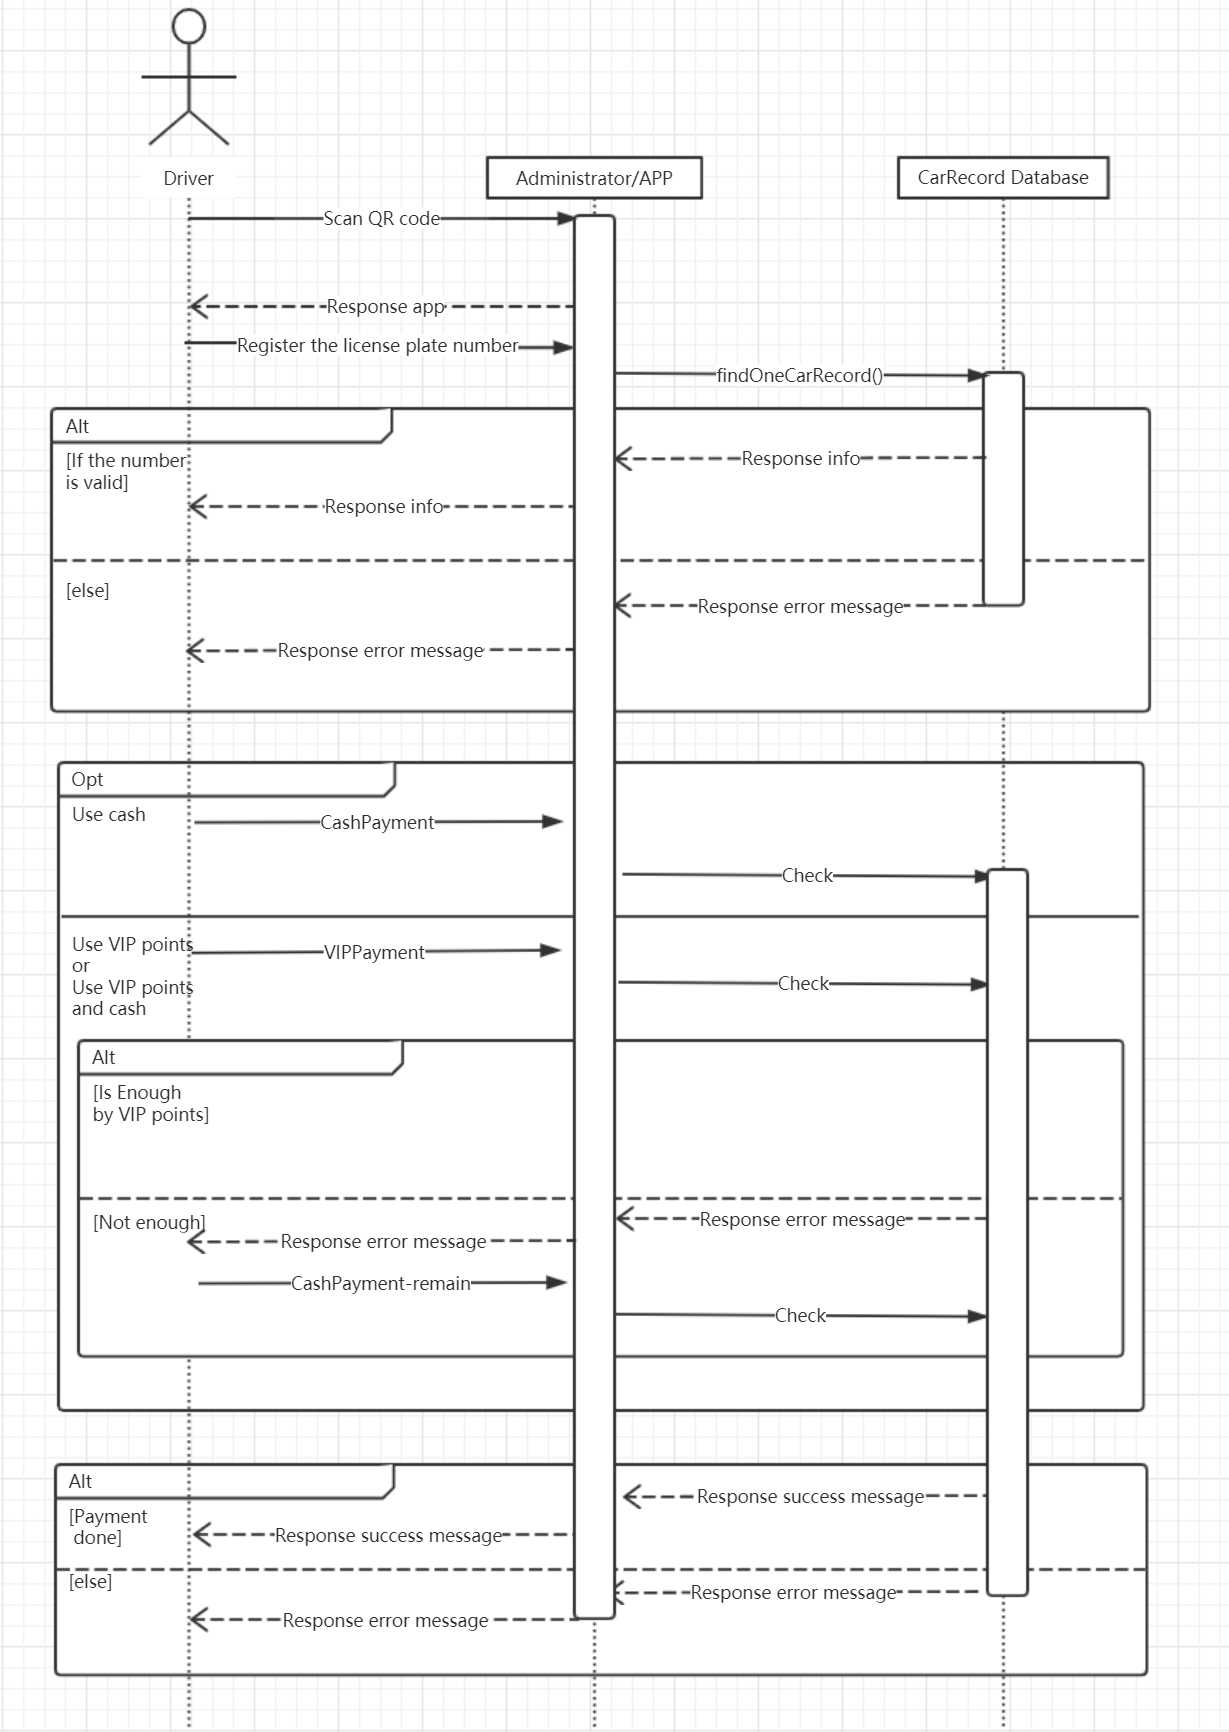
\includegraphics[width=0.4\textwidth]{Fig3.png}\\
  \caption{Trie
}\label{straddltimeScale}
\end{figure}

And the function \emph{make\_fail} do this thing:

\begin{figure}[H]
  \centering
  % Requires \usepackage{graphicx}
  \includegraphics[width=0.4\textwidth]{Fig4.png}\\
  \caption{make_fail
}\label{straddltimeScale}
\end{figure}

\section{Performance Analytics}

\subsection{Dataset}
In the first stage, I cannot pass the pretest for my first submission. So that I creat some given chessboard for my AI and step by step debugging to find bugs. For convenience, I wrote a visual program that could display a chess board and I could play chess on it to simulate the AI against me, and at the same time, I could also watch the AI data change. Here are some dataset and the chessboard I built:

\begin{figure}[H]
  \centering
  % Requires \usepackage{graphicx}
  \includegraphics[width=0.4\textwidth]{Fig5.png}\\
  \caption{blank first, blank win(Alive3)
}\label{straddltimeScale}
\end{figure}

\begin{figure}[H]
  \centering
  % Requires \usepackage{graphicx}
  \includegraphics[width=0.4\textwidth]{Fig6.png}\\
  \caption{white first, white win(Alive3 + Jump3)
}\label{straddltimeScale}
\end{figure}

From this data, I pass all the pretest and find how adjust the parameter of pattern's score.

\subsection{Performance measure}
To keep track of time, I added some time keeping code to my AI code. After each run of the dataset I built myself, I let the program to output the total test time, the time spent on each test sample:

\begin{figure}[H]
  \centering
  % Requires \usepackage{graphicx}
  \includegraphics[width=0.4\textwidth]{Fig7.png}\\
  \caption{Running time
}\label{straddltimeScale}
\end{figure}

Due to this way, I get the average time for the dataset, but it is not the worth case. The worth case is the AI should run the while minimax search tree with no $\alpha$-$\beta$ pruning. But I think my AI could not meet this case because it select top 5 steps in each depth and sort them. It is benefit for the $\alpha$-$\beta$ pruning so that the running time is much less than the worth case.

\subsection{Hyperparameters}

\begin{itemize}
    \item 
    For the first stage, pass 25 pretest is my goal. So I set a basic score table for each pattern. It just follows Five > Alive4 > Alive3 > Ruch4 > Jump4 > jump3 > Alive2 > Rush3 > Rush2
\end{itemize}
\begin{itemize}
    \item 
    For the second stage, That score table is too week to fight with other AI. So that I refined each pattern's score and their combination. For example, Alive3 + Jump3 = ALive4. And I find some special case:
    
    \begin{figure}[H]
      \centering
      % Requires \usepackage{graphicx}
      \includegraphics[width=0.4\textwidth]{Fig8.png}\\
      \caption{Running time
    }\label{straddltimeScale}
    \end{figure}
    
    For my evaluation function, it just thinks black only have a jump4 and it is not a winning game. In fact, it is a winning game for black.
    
    When I fix those bugs, my rank is up. When the rank is top 20, it is not easy to fight against all the AI, so I play will the AI by hand or "playto". Then play chess on their weaknesses.
\end{itemize}
\begin{itemize}
    \item 
    For the third stage, I think the server runs the AI of many classmates at the same time.The computing power of the server will decrease significantly.Therefore, I adjusted the time limit of my code to make it run a little faster, and when the time was running out, I reduced the accuracy and greatly improved the speed, so as to avoid the failure caused by overtime.
\end{itemize}

\subsection{Experimental results}
Before I did that:

\begin{figure}[H]
  \centering
  % Requires \usepackage{graphicx}
  \includegraphics[width=0.4\textwidth]{Fig9.png}\\
  \caption{Rank37
}\label{straddltimeScale}
\end{figure}

After I did that:

\begin{figure}[H]
  \centering
  % Requires \usepackage{graphicx}
  \includegraphics[width=0.4\textwidth]{Fig10.png}\\
  \caption{Rank4
}\label{straddltimeScale}
\end{figure}

The final score:

\begin{figure}[H]
  \centering
  % Requires \usepackage{graphicx}
  \includegraphics[width=0.4\textwidth]{Fig11.png}\\
  \caption{Rank4
}\label{straddltimeScale}
\end{figure}

\subsection{Conclusion}
The biggest disadvantage is that I use DFS when using minimax search tree.In fact, BFS is probably better, because if something goes over time, the worst case for DFS is that the program doesn't add any points to the board, or it finds a point where the score isn't that high.The BFS outputs the current optimal result.\\

Second, because of the time and the difficulty of code implementation, I did not write the hash substitution table. With BFS, the depth of minimax search tree can be greatly increased by recording the cases that have been run in the hash table.\\

Third, I think my strategy to deal with the time limit is worth learning. Thanks to the parameter adjustment in the third stage, my score in the third stage is higher than that in the second stage.

Finally, my kill chess so bad that it cannot pass the pretests. Kill chess is a very smart method. As long as you can find a continuous Alive3 or Rush4, go them continuously and the enemy cannot defense it.

\section*{Acknowledgements}
Thanks for the platform SA built. Although it has so many bugs, it spent two weeks of great nights with us.

\bibliographystyle{ieeetr}
\bibliography{references}

\end{document}
